נתונים $n$ אינטרוולים
$A = \{(a_1, b_1), \ldots, (a_n, b_n)\}$, 
$a_i, b_i \in \mathbb{R}_+$
וכן 
$a_i \leq b_i$
רוצים למצוא תת קבוצה בגודל מקסימלי
$I \subseteq A$
כך שהאינטרוולים ב-$I$ זרים בזוגות, כלומר לכל 
$i \leq j$, 
כך ש-%
$(a_i, b_i), (a_j, b_j) \in I$
אחד התנאים מתקיים:
$b_i < a_j$
או ש-%
$a_i > b_j$.
דוגמה:

\begin{center}
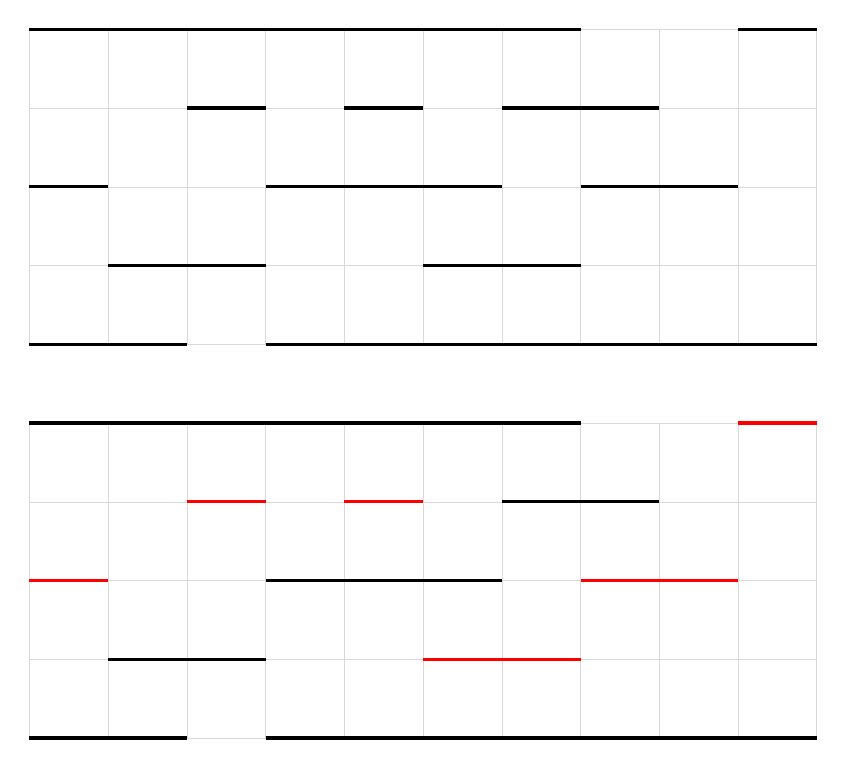
\begin{tikzpicture}[very thick]
\draw[very thin, gray!30] (0,0) grid (10, 4);
\draw (0,0) -- (2,0);
\draw (3,0) -- (10,0);

\draw (1,1) -- (3,1);
\draw (5,1) -- (7,1);

\draw (0,2) -- (1,2);
\draw (3,2) -- (6,2);
\draw (7,2) -- (9,2);

\draw (2,3) -- (3,3);
\draw (4,3) -- (5,3);
\draw (6,3) -- (8,3);

\draw (0,4) -- (7,4);
\draw (9,4) -- (10,4);

\begin{scope}[yshift=-5cm]
\draw[very thin, gray!30] (0,0) grid (10, 4);
\draw (0,0) -- (2,0);
\draw (3,0) -- (10,0);

\draw (1,1) -- (3,1);
\draw[red] (5,1) -- (7,1);

\draw[red] (0,2) -- (1,2);
\draw (3,2) -- (6,2);
\draw[red] (7,2) -- (9,2);

\draw[red] (2,3) -- (3,3);
\draw[red] (4,3) -- (5,3);
\draw (6,3) -- (8,3);

\draw (0,4) -- (7,4);
\draw[red] (9,4) -- (10,4);
\end{scope}

\end{tikzpicture}
\end{center}

אלגוריתם חמדן:
\begin{enumerate}
\item
אתחול:
$I \leftarrow \emptyset$, 
$b \leftarrow 0$
\item
עבור כל אינטרוול 
$(a_i, b_i)$
בסדר לא יורד של ערכי 
$b_i$:
	\begin{enumerate}
	\item
	אם 
	$a_i \geq b$
		\begin{enumerate}
		\item
		$I \leftarrow I \cup \{(a_i, b_i)\}$
		\item
		$b \leftarrow b_i$				
		\end{enumerate}

	\end{enumerate}
\end{enumerate}

הוכחת נכונות: נוכיח את הטענה הבאה, בכל פעם שהאלגוריתם מוסיף אינטרוול אז קיים שיבוץ אופטימלי
שמכיל את $I$ 

